\documentclass[journal]{IEEEtran}
%\documentclass{IEEEtran}
	\usepackage{graphicx}
	\usepackage{caption}
	\usepackage{hyperref}
    \usepackage{float}
    
\begin{document}

\title{Group 67 - Research Paper}
\author{Deep Learning for Object Recognition on a Mobile Robot\\
Julian Weisbord, Miles McCall, Michael Rodriguez \\
Oregon State University \\
CS 463 Spring 2018 \\
}
\maketitle

\begin{abstract}
	The research paper is the write up of our research findings. It includes the methods and technologies we tested in our project and the results from those experiments. This document acts as the conclusion to the research aspect of our project.
\end{abstract}

\begin{IEEEkeywords}
	Deep Learning, Online Learning, Object Recognition, Mobile Robot
\end{IEEEkeywords}

\tableofcontents

\listoffigures

\section{Introduction \& Background}
	Our project is research oriented, which differs in certain ways from creating a deliverable product like other senior design projects. While one of the main goals of the project is to create a fully functional software pipeline as part of our deliverables, we were also setting out to answer scientific questions and generate our own hypotheses involving the different technologies in our project. 
	
	The software pipeline consists of several main programs that interact with each other to collect and process our image data. These main programs encapsulate each task our overarching classification system requires, and hence represent the main logical steps in our pipeline. 
	
	For each of these programs, our team wanted to implement the best performing technology within our limits we could. To accomplish this, our initial research investigated each step and compared varying technologies, techniques, and resources available to us. We hypothesized which solutions would fit our project the best, and factored values such as cost-benefit analyses and the potential to scale technologies as our classification model grows into our predictions. 
	
	Improving upon the performance of the lab's current classification model is one of the main goals of our pipeline, so finding measurable metrics to evaluate performance is important to the success of our project. By measuring the training speed, training and validation accuracy, and classification success rates, we can compare and contrast the current classification model to our model. These values are easily recorded while the classification program runs and be plotted to observe patterns in the results. 
\section{Hypothesis}	
\section{Areas of Research}
	%While the main goal of our project was to create a fully functional software pipeline, we incorporated research into every component of the pipeline. The problem of sequential online learning is not solved by one perfect algorithm or software library
	\subsection{Hardware Solutions}  
	 	\subsubsection{Robot Platforms}
	 	\subsection{Computing Resources}
	\subsection{Data Gathering}
	\subsection{Neural Network Model}
	\subsection{Sequential Online Learning}
  
\section{Results} 
	\subsection{Figures}
		\begin{figure}[H]
			\begin{center}
				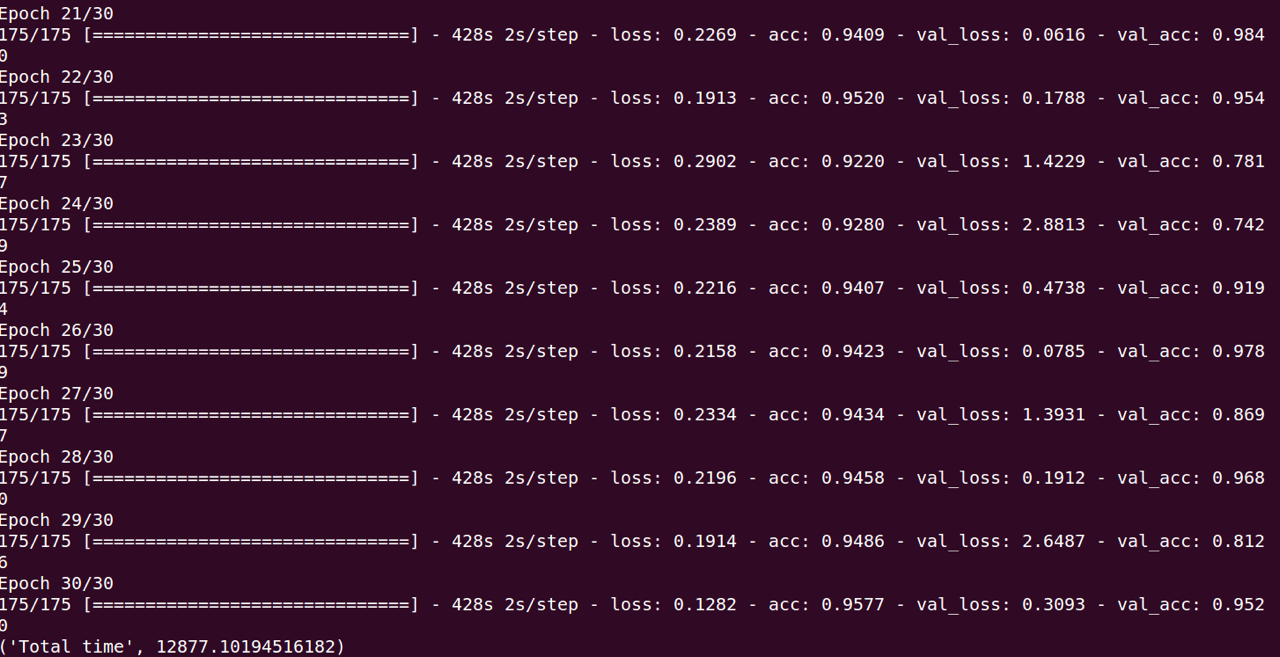
\includegraphics[width=\linewidth]{pictures/results.png}
				\caption{Accuracy Training}
			\end{center}
		\end{figure}
		\begin{figure}[H]
			\begin{center}
				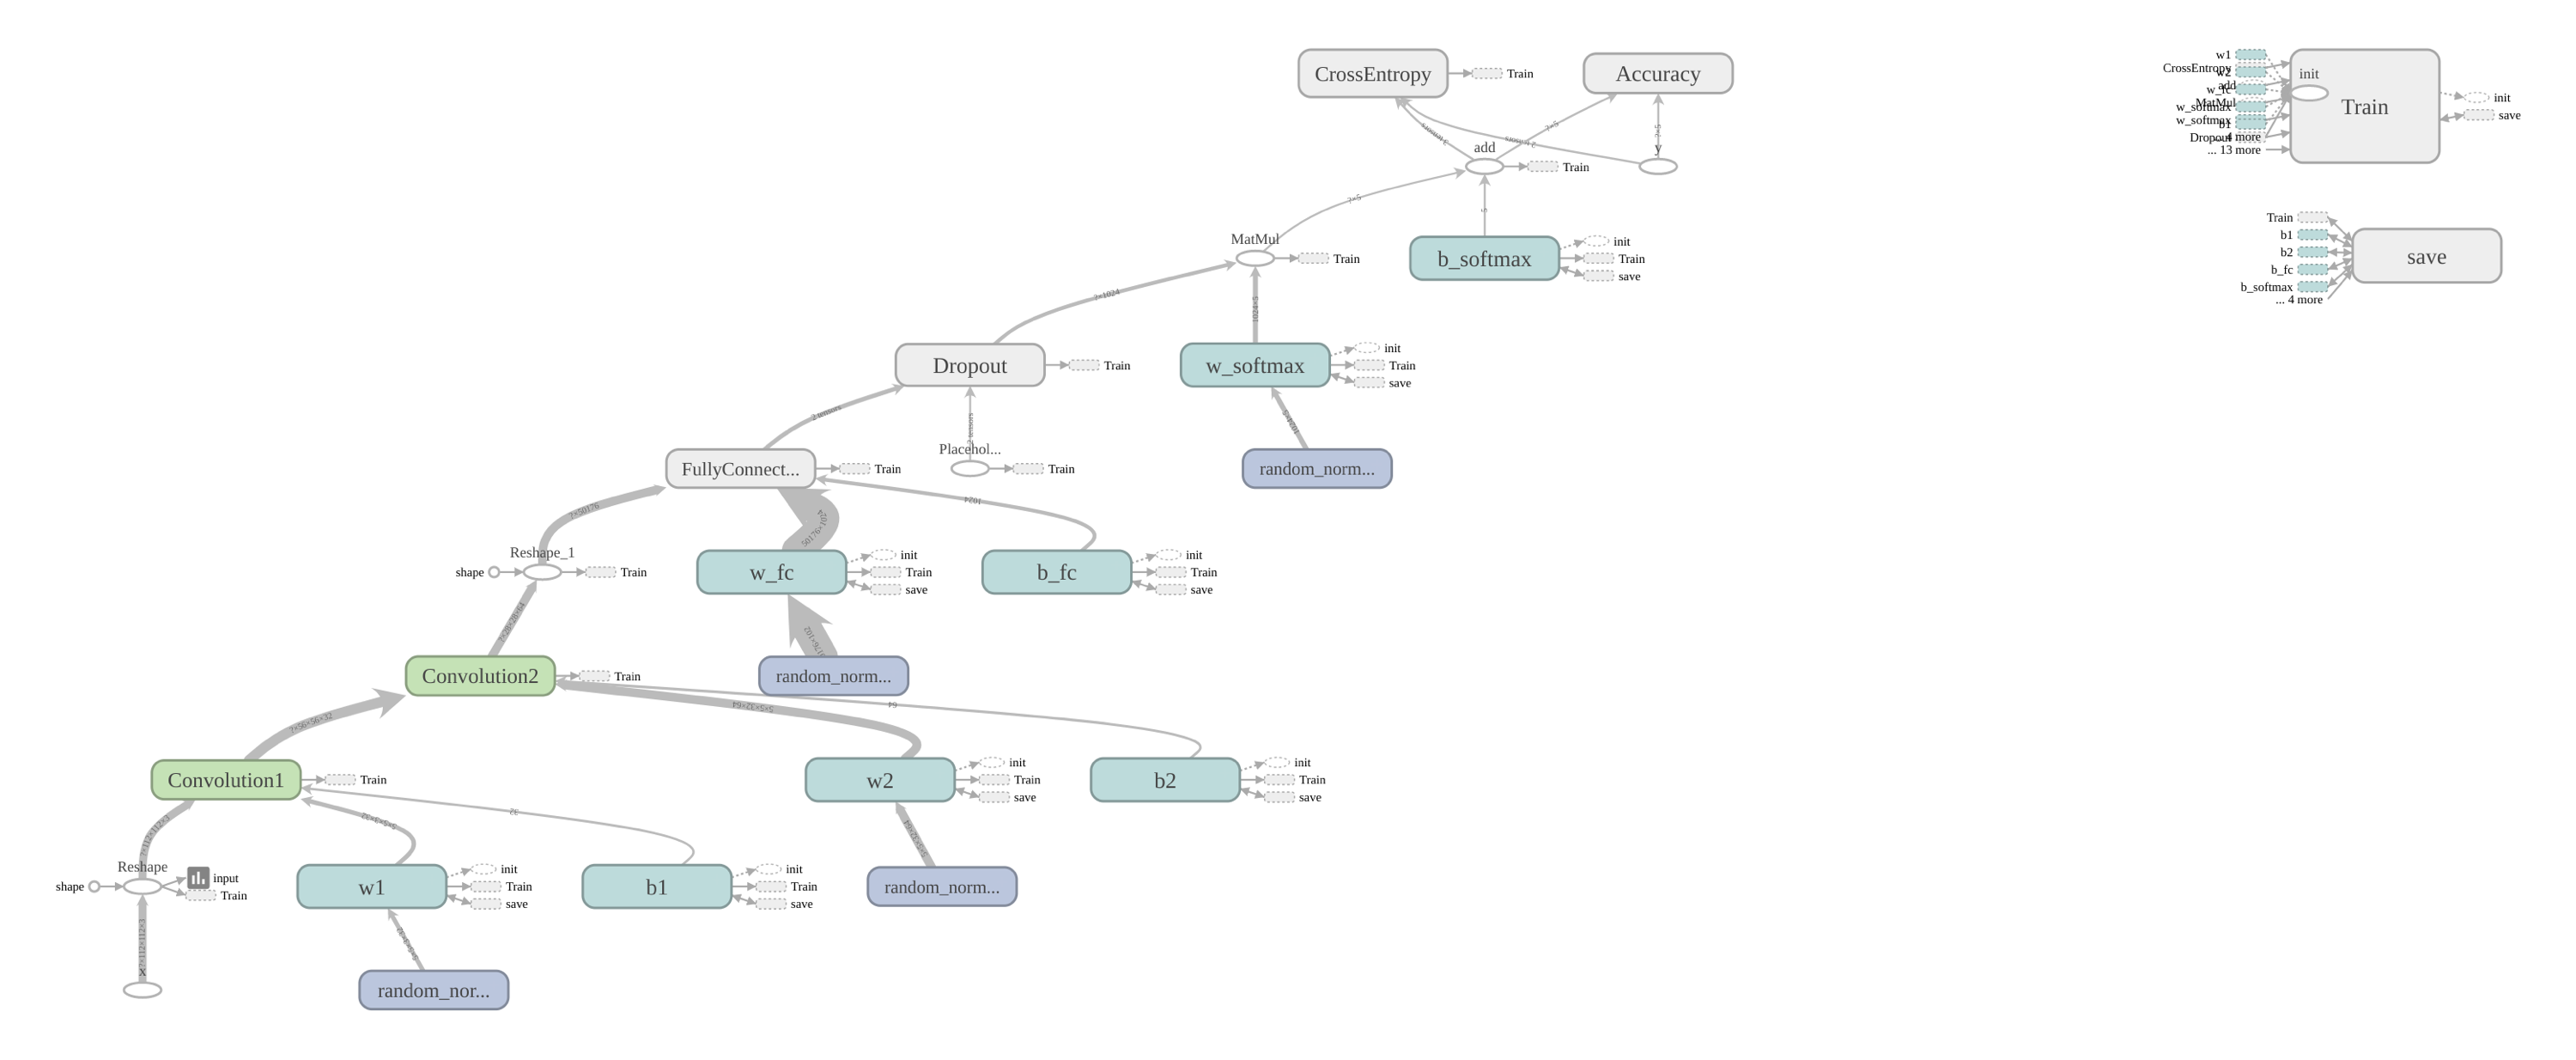
\includegraphics[width=\linewidth]{pictures/model.png}
				\caption{Network Model}
			\end{center}
		\end{figure}
	
	\subsection{Data Analysis}

\section{Conclusion}

\appendix
\newpage
%\bibliography{research}
%\bibliographystyle{IEEEtran}
\end{document}